\documentclass[margin=0pt]{standalone}
\usepackage[romanfamily=casual,lucidasmallscale, nofontinfo]{lucimatx}
%\usepackage[romanfamily=bright-osf, stdmathdigits=true,lucidasmallscale, nofontinfo]{lucimatx}
\linespread{1.04}	%  this value suits  scale=0.9  or lucidasmallscale
\usepackage{tikz}
\begin{document}%
  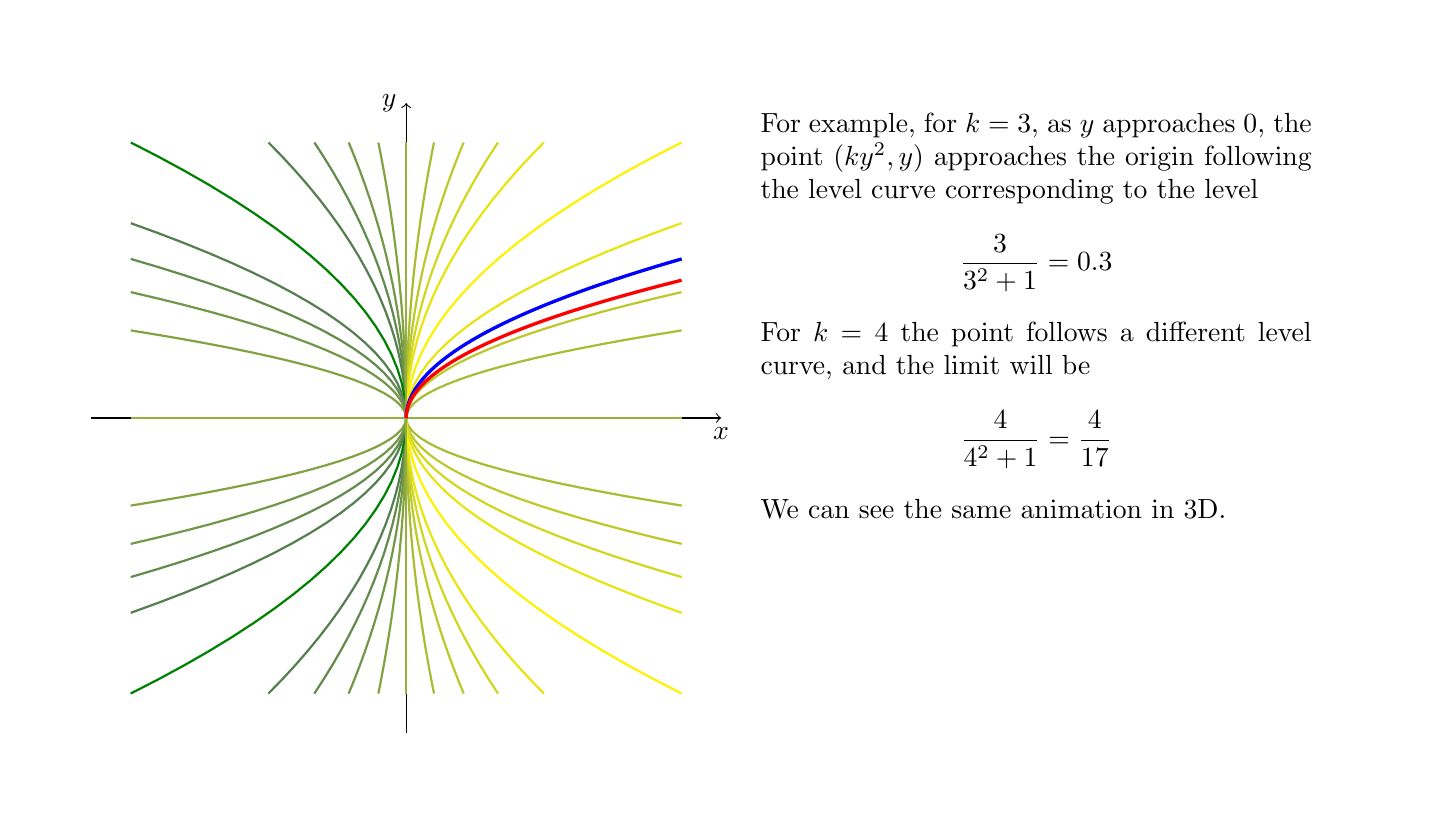
\begin{tikzpicture}
      \draw[white] (-8.8,-4.94) rectangle (8.8,4.95);
      \begin{scope}[xshift=-4cm]
          \def\scale{3.5}
          \colorlet{darkgreen}{green!50!black};
          \draw[thin,->] (-4,0) -- (4,0)node[below]{$x$};
          \draw[thin,->] (0,-4) -- (0,4)node[left]{$y$};
          \foreach \i in {-4,...,-1}{
          \pgfmathsetmacro{\k}{.1*\i};
          \pgfmathsetmacro{\coefa}{(1-sqrt(1-4*(\k)^2))/(2*\k)};
          \pgfmathsetmacro{\color}{10*(5+\i)};
          \draw[thick,color=yellow!\color!darkgreen] plot[domain=-1:1,samples=40] ({\scale*\coefa*(\x)^2},\scale*\x);
          }
          \draw[thick,color=darkgreen] plot[domain=-1:1,samples=40] ({-\scale*(\x)^2},\scale*\x);
          \begin{scope}
              \clip (-\scale,-\scale) rectangle (\scale,\scale);
              \foreach \i in {-4,...,-1}{
              \pgfmathsetmacro{\k}{.1*\i};
              \pgfmathsetmacro{\coefa}{(1+sqrt(1-4*(\k)^2))/(2*\k)};
              \pgfmathsetmacro{\color}{10*(5+\i)};
              \pgfmathsetmacro{\dom}{1/sqrt(-\coefa)}
              \draw[thick,color=yellow!\color!darkgreen] plot[domain=-\dom:\dom,samples=40] ({\scale*\coefa*(\x)^2},\scale*\x);
              }
          \end{scope}
          \foreach \i in {1,...,4}{
          \pgfmathsetmacro{\k}{.1*\i};
          \pgfmathsetmacro{\coefa}{(1-sqrt(1-4*(\k)^2))/(2*\k)};
          \pgfmathsetmacro{\color}{10*(5+\i)};
          \draw[thick,color=yellow!\color!darkgreen] plot[domain=-1:1,samples=40] ({\scale*\coefa*(\x)^2},\scale*\x);
          }
          \draw[thick,color=yellow] plot[domain=-1:1,samples=40] ({\scale*(\x)^2},\scale*\x);
          \begin{scope}
              \clip (-\scale,-\scale) rectangle (\scale,\scale);
              \foreach \i in {1,...,4}{
              \pgfmathsetmacro{\k}{.1*\i};
              \pgfmathsetmacro{\coefa}{(1+sqrt(1-4*(\k)^2))/(2*\k)};
              \pgfmathsetmacro{\color}{10*(5+\i)};
              \pgfmathsetmacro{\dom}{1/sqrt(\coefa)}
              \draw[thick,color=yellow!\color!darkgreen] plot[domain=-\dom:\dom,samples=40] ({\scale*\coefa*(\x)^2},\scale*\x);
              }
          \end{scope}
          \draw[thick,color=yellow!50!darkgreen] (-\scale,0) -- (\scale,0);
          \draw[thick,color=yellow!50!darkgreen] (0,-\scale) -- (0,\scale);
          \begin{scope}
              \clip (-\scale,-\scale) rectangle (\scale,\scale);
              \pgfmathsetmacro{\k}{.3};
              \pgfmathsetmacro{\coefa}{(1+sqrt(1-4*(\k)^2))/(2*\k)};
              \pgfmathsetmacro{\dom}{1/sqrt(\coefa)}
              \draw[very thick,color=blue] plot[domain=0:\dom,samples=40] ({\scale*\coefa*(\x)^2},\scale*\x);
              \pgfmathsetmacro{\k}{4/17};
              \pgfmathsetmacro{\coefa}{(1+sqrt(1-4*(\k)^2))/(2*\k)};
              \pgfmathsetmacro{\dom}{1/sqrt(\coefa)}
              \draw[very thick,color=red] plot[domain=0:\dom,samples=40] ({\scale*\coefa*(\x)^2},\scale*\x);
          \end{scope}
      \end{scope}
      \node[below] at (4,4) {%
      \begin{minipage}[t]{7cm}
          For example, for $k = 3$, as $y$ approaches $0$, the point $(ky^2,y)$
          approaches the origin following the level curve corresponding to the
          level 
          \[\frac{3}{3^2 + 1} = 0.3\]
          For $k = 4$ the point follows a different level curve, and the limit
          will be \[\frac{4}{4^2+1} = \frac{4}{17}\]

          We can see the same animation in 3D.
      \end{minipage}%
      };
  \end{tikzpicture}%
\end{document}
